\usepackage{graphicx}
\usepackage{luatexja-fontspec}
\usepackage{caption}
\usepackage{amsmath,amssymb,bm,braket}
\usepackage[english]{babel}
\usepackage{multicol}
\usepackage{titlesec}
%\usepackage{gnuplot-lua-tikz}
\usepackage[top=20truemm,bottom=20truemm,left=20truemm,right=20truemm]{geometry}
\usepackage{array}
\usepackage{upgreek}
\usepackage{fancyhdr}
\renewcommand{\refname}{}
\usepackage{listings,jvlisting}
\usepackage{tikz}
\usepackage[thmmarks,amsmath]{ntheorem}
\usepackage[version=3]{mhchem}
\usetikzlibrary{external}
\tikzexternalize
\lstset{
  basicstyle={\ttfamily},
  identifierstyle={\small},
  commentstyle={\smallitshape},
  keywordstyle={\small\bfseries},
  ndkeywordstyle={\small},
  stringstyle={\small\ttfamily},
  frame={tb},
  breaklines=true,
  columns=[l]{fullflexible},
  numbers=left,
  xrightmargin=0pt,
  xleftmargin=3pt,
  numberstyle={\scriptsize},
  stepnumber=1,
  numbersep=1pt,
  lineskip=-0.5ex
}
\captionsetup[figure]{format=plain, labelformat=simple, labelsep=quad,labelfont=bf,name={Fig.}}
\captionsetup[table]{format=plain, labelformat=simple, labelsep=quad,labelfont=bf}
\parindent = 0pt
%[BoldFont=HGSMinchoE]{MSMincho}[BoldFont=HiraMinProN-W6]{HiraMinPro-W3}
\titleformat{\section}{\normalfont\fontsize{9}{10}\bfseries\fontspec{Times New Roman}}{\thesection.}{1em}{}
\usepackage[backend=biber,sorting=none,style=numeric,maxnames=99,minnames=1]{biblatex}
\addbibresource{utility/REFERENCES.bib}
\defbibheading{bibliography}[\refname]{%
  \section*{REFERENCES}%
  \vspace{-7pt}  % ここで空白を調整。お好みの値に変更してください。
}
\newfontfamily\subsectionfont{Times New Roman} % サブセクション用フォント
\titleformat{\subsection}
  {\normalfont\large\bfseries} % サブセクションのフォントを指定
  {\thesubsection}{1em}{}
\renewbibmacro{in:}{}
\renewbibmacro*{journal+issuetitle}{%
  \addcomma\space% カンマとスペースを追加
  \usebibmacro{journal}%
  \setunit*{\addspace}%
  \usebibmacro{volume+number+eid}%
  \setunit{\addspace}%
  \printfield{note}%
  \newunit
}
\renewbibmacro*{volume+number+eid}{
  \printfield{volume}%
  \setunit*{\addnbspace}%
  \printfield{number}%
  \setunit{\addcomma\space}%
  \printfield{eid}
}
\DeclareFieldFormat[article]{volume}{\textbf{#1}}
\DeclareFieldFormat[article]{pages}{#1}
\DeclareFieldFormat{journaltitle}{#1}
\usepackage{hyperref}
\renewenvironment{abstract}{\par\noindent}{\par}
%\pagenumbering{gobble}
\usepackage{docmute}
\usepackage{setspace}
\usepackage{titlesec} % 見出しのカスタマイズ用

% セクションのフォーマットをカスタマイズ
\titleformat{\section}
  {} % フォントサイズとスタイル
  {\Large\bfseries\thesection\ \ }               % 番号の前の内容(空白)
  {0em}            % 番号とタイトルの間の間隔
  {\Large\bfseries}


\theoremstyle{plain}
\theoremheaderfont{\normalfont\bfseries}
\theorembodyfont{\itshape}   % 本文を斜体に
\theoremseparator{.}         % タイトルと本文の区切りを「.」に設定
\newtheorem{definition}{Definition}
\begin{document}
\frenchspacing
\twocolumn[
\begin{@twocolumnfalse} % ここで一時的に1段組み
  \centerline{\fontsize{14}{18}\selectfont\bfseries  擬似3次元表面符号のための格子手術}
  \vspace{5pt}
  \centerline{\fontspec{Arial}[BoldFont=Arial Bold]\fontsize{12}{18}\textbf{Lattice Surgery for Pseudo-Three-Dimentional Surface Code}}
  \centerline{\fontsize{10}{18} 物理情報工学科 山本研究室 学籍番号:62115799 平井優我}
  \vspace{6pt}
  \begin{abstract}
    Abstract: Quantum computers promise significant advantages, but high qubit error rates remain a challenge. The surface code, combined with a looped pipeline in semiconductor quantum computers, enables pseudo-3D surface codes that improve lattice surgery and magic state distillation. Our pseudo-3D results show notable improvements, significantly reducing both the longest and average distances in lattice surgery, and enabling a more efficient magic factory.
  \end{abstract}
  \vspace{2pt}
  \leftline{Keywords: quantum comuputer, quantum error correction, quantum dot, computer architecture}
  \vspace{8pt}
\end{@twocolumnfalse}]
  \section{INTRODUCTION}
  \vspace{-8pt}
  \ \ Lattice Surgery\textsuperscript{\cite{horsman2012}} is a known method for performing gate operations on logical qubits encoded by surface codes while simultaneously correcting errors. By surgery operations, each encoded in separate surface codes, can perform gate operations by using the ancillary qubits located between them. In semiconductor quantum computers realized using quantum dots, it is possible to create a one-dimensional looped pipeline\textsuperscript{\cite{cai2023}}. By employing such a structure, a pseudo-three-dimensional surface code, resembling multiple stacked layers of surface codes, can be constructed \\Fig.\ \ref{figure1}(a). This architecture is being explored to improve the parallelization of lattice surgery between multiple logical qubits, which has been a bottleneck in previous systems. Additionally, efforts will be made to optimize another bottleneck, the efficiency of magic state distillation\textsuperscript{\cite{litinski2019game}\cite{litinski2019magic}} through improved Magic Factories.
  \section{METHOD}
  \vspace{-8pt}
  \ \ In this paper, we define a surface code that encodes a single logical qubit with a code distance of $d$ as a patch, and $d$ rounds of syndrome measurements as one code beat. In three-dimensional lattice surgery, movements between floors must be carefully considered. In two-dimensional setups, any two patches can be connected within a single code beat, with the time dependent solely on gate operations and measurements, independent of distance. However, in three dimensions, moving between floors requires transversal-CNOT gates, and the time is proportional to the inter-floor distance. We assume the ability to move up or down by two floors consecutively. In the looped pipeline architecture, moving upstairs from the top floor allows descending to the bottom floor, and vice versa. Based on these assumptions, we propose a framework to improve lattice surgery efficiency and magic state distillation.
  \begin{figure}[t]
    \centering
    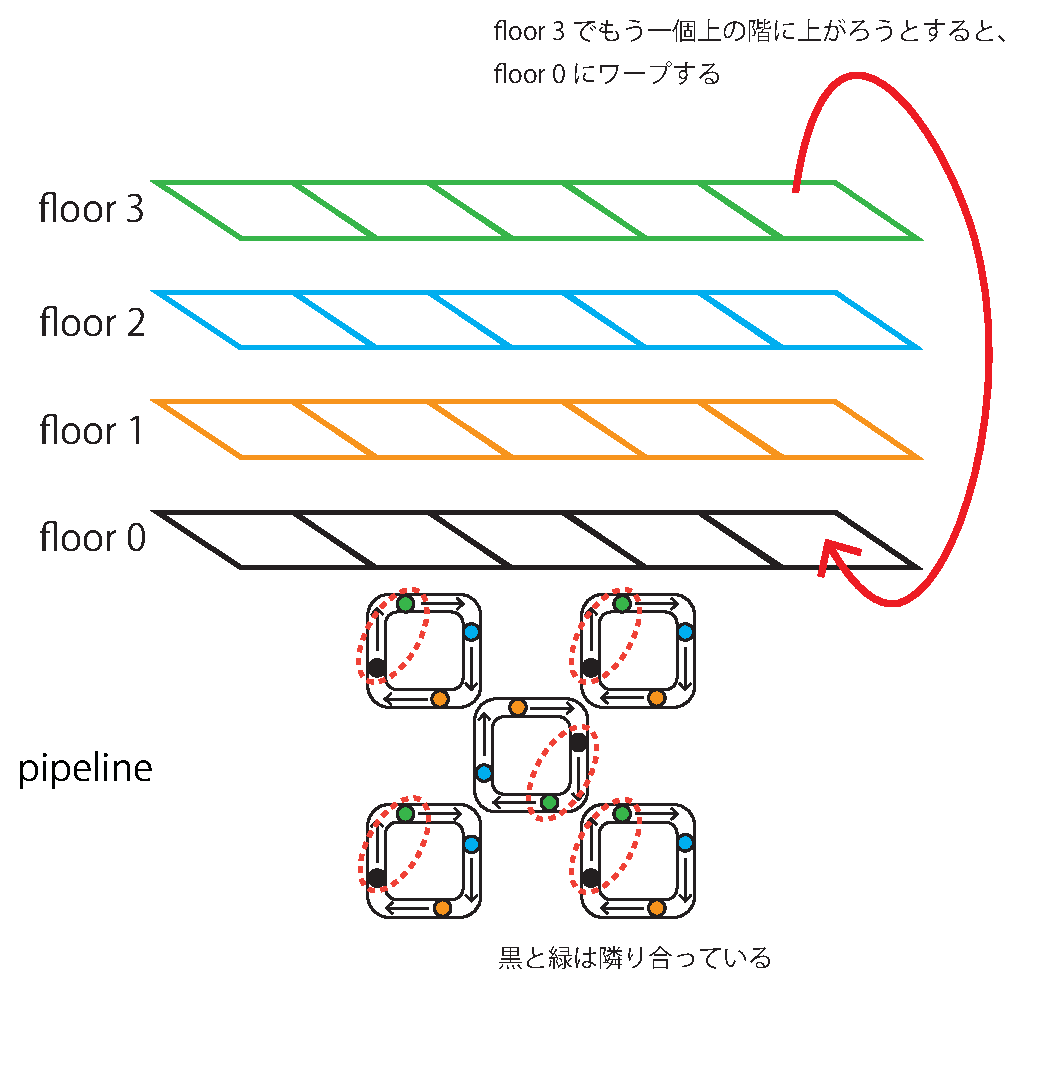
\includegraphics[scale=0.30]{figure/figure1.eps}
    \vspace{-10pt}\caption{(a) left: Looped pipeline architecture, right:  Hierarchical structure of the 3D surface code. (b) Distance of surgery operations in the 2D Heisenberg model Top: 2D, Bottom: 3D. (c) Design of the magic factory.}
    \label{figure1}
    \vspace{-15pt}
  \end{figure}
  \section{RESULTS}
  \vspace{-8pt}
  \ \ By applying lattice surgery in three dimensions, significant improvements were observed compared to the two-dimensional case, as illustrated in Fig.\ \ref{figure1}(b). The graph shows that in 2D lattice surgery, many operations exceeded a distance of 100, whereas in 3D lattice surgery, even the longest distance remained below 100. Furthermore, the average distance was reduced from 21.02 in 2D to 8.43 in 3D. Figure.\ \ref{figure1}(c) presents the design of the magic factory. Using this configuration, a single magic state can be generated in 8 code beats on a 3D surface code.
  \section{CONCLUSION AND FUTURE WORK}
  \vspace{-8pt}
  \ \ The implementation of the 3D surface code significantly reduces routing overhead in lattice surgery. However, while the distance for individual surgery operations has been shortened, the increased parallelism leads to a larger number of physical qubits requiring decoding within a single code beat. This imposes a substantial computational burden on classical systems, highlighting the need for further optimization. Additionally, the optimal placement of logical qubits on the 3D surface code used in this study remains unaddressed. Future work will focus on optimizing this placement and conducting a detailed analysis of the proposed magic factory's performance within lower-layer pipeline architectures.


\printbibliography
\end{document}
